\documentclass[english]{article}

%\usepackage[T1]{fontenc}
\usepackage[latin9]{inputenc}
\usepackage[letterpaper]{geometry}
\geometry{verbose,tmargin=1in,bmargin=1in,lmargin=1in,rmargin=1in}
\usepackage{babel}
\usepackage{amsmath}
\usepackage{amssymb}
\usepackage{capt-of}
\usepackage{graphicx}
\usepackage{color}
\usepackage{latexsym}
\usepackage{xspace}
\usepackage{pdflscape}
\usepackage[hyphens]{url}
\usepackage[colorlinks]{hyperref}
\usepackage{enumerate}
\usepackage{ifthen}
\usepackage{float}
\usepackage{array}
\usepackage{tikz}
\usepackage{multirow} 
\usetikzlibrary{shapes}
\usepackage{algorithm2e}
\usepackage{listings}
\usepackage{verbatim}
%%%% HW instructions / collaboration text

\newcommand{\HWPoliciesmix}{
\paragraph*{Instructions.} {\bf This homework contains two parts. Part A is written assignment and Part B is MATLAB programming assignment.}
}

\newcommand{\HWPolicies}{
\paragraph*{Instructions.} 
Please write up your responses to the following problems clearly and
concisely. We encourage you to write up your responses using \LaTeX{};
we have provided a \LaTeX{} template, available on Canvas, to
make this easier. {\bf Submit your answers in PDF form to Canvas. We will not accept paper copies of the homework.}

\paragraph*{Collaboration.} 
You are allowed and encouraged to work together. You may discuss the
homework to understand the problem and reach a solution in groups up
to size {\bf four students.} However, {\em each student must write
  down the solution independently, and without referring to written
  notes from the joint session. {\bf In addition, each student must
    write on the problem set the names of the people with whom you
    collaborated.}} You must understand the solution well enough in
order to reconstruct it by yourself. (This is for your own benefit:
you have to take the exams alone.)
}
\newcommand{\ProgrammingPolicies}[1]{
\paragraph*{Instructions.} 
This is a MATLAB programming assignment. This assignment consists of
multiple parts. Portions of each part will be graded automatically,
and you can submit your code to be automatically checked for
correctness to receive feedback ahead of time.

We are providing you with codebase / templates / dataset that you will
require for this assignment. Download the file {\tt hw#1\_kit.zip}
from Canvas {\bf before} beginning the assignment.  {\bf Please
  read through the documentation provided in ALL Matlab files before
  starting the assignment.} The instructions for submitting your
homeworks and receiving automatic feedback are online on the wiki:

\begin{center}
\url{http://alliance.seas.upenn.edu/~cis520/wiki/index.php?n=Resources.HomeworkSubmission}
\end{center}

\paragraph*{Collaboration.} 
For this programming assignment, you are allowed to work in pairs, but no more than 2. Each group
is required to submit {\bf ONCE} only. {\bf The LOWEST grade will be recorded for multiple submissions.}
Be sure to include your pennkeys and names in the {\it Group.txt} file.
Failure to do so will result in a failure in the grading process. 
{\bf We will be using automatic checking software to detect blatant copying of other student's assignments, so,
please, don't do it.}
}

%%%% CUSTOM COMMANDS FOR FORMATTING EXAMS/HOMEWORKS
\newcounter{section_points}[section]
\newcounter{header_points}[section]
\newcounter{total_points}

\newcommand{\hpoints}[1]{
  \setcounter{header_points}{#1}
  \textbf{[#1 points]}
}

\newcommand{\points}[1]{
  \addtocounter{section_points}{#1}
  \addtocounter{total_points}{#1}
  \textbf{[#1 
    \ifthenelse{\equal{#1}{1}}
    {point}{points}]}
}

\newcommand{\bpoints}[1]{
  \textbf{[#1 
    \ifthenelse{\equal{#1}{1}}
    {point}{points}]}
}


\newcommand{\point}{\textbf{[1 point]}}

\newboolean{ShowSolutions}
\newcommand{\Mistake}[2]{
  \ifthenelse{\boolean{ShowSolutions}}
  {\paragraph{\bf $\blacksquare$ COMMON MISTAKE #1:} {\sf #2} \bigskip}
  {}
}

\newcommand{\Solution}[2]{
  \ifthenelse{\boolean{ShowSolutions}}
    {
      \paragraph{\bf $\bigstar $ SOLUTION:} { \sf
        #1} \bigskip
    }
    { 
      #2
    } %} \vspace{1.5in}}
}
\newcommand{\out}[1]{}

\newboolean{ShowPointsInfo}

\newcommand{\PointStats}[0]{
  \ifthenelse{\boolean{ShowPointsInfo}}
  {
    \begin{center}

      \begin{tabular}{rl}
        \hline
        Stated Points: & \arabic{header_points} \\
        Section Points: & \arabic{section_points} \\
        Total Points So Far: & \arabic{total_points} \\
        \hline 
        \multicolumn{2}{c}{
          
          \ifthenelse{
            \equal{\value{section_points}}{\value{header_points}}
          }{CORRECT TOTAL}
          {{\bf INCORRECT TOTAL}}
          }
          \\
        \hline
      \end{tabular}
    \end{center}
  }{}
}

\newcounter{blankcount}
\newcommand{\myrepeat}[2] {
\setcounter{blankcount}{1}
\whiledo{\value{blankcount} < #1}{
#2
\addtocounter{blankcount}{1}
}
}

\newcommand{\blank}[1]{\underline{\myrepeat{#1}{\qquad}}}


%%%% CUSTOM MATH GOES HERE

\newcommand{\ind}[1]{\mathbf{1}\left(#1\right)}
\renewcommand{\Pr}{\mathbf{Pr}\xspace}
\newcommand{\Bern}{\textsf{Bernoulli}\xspace}
\newcommand{\sign}{\textsf{sign}}

\newcommand{\E}{\mathbf{E}}
\newcommand{\bx}{\mathbf{x}}
\newcommand{\bX}{\mathbf{X}}
\newcommand{\by}{\mathbf{y}}
\newcommand{\bY}{\mathbf{Y}}
\newcommand{\bz}{\mathbf{z}}
\newcommand{\bw}{\mathbf{w}}
\newcommand{\bl}{\mathbf{\ell}}
\newcommand{\vc}[1]{\mathbf{#1}}

\newcommand{\Hypo}{\mathcal{H}}
\newcommand{\XX}{\mathcal{X}}
\newcommand{\cD}{\mathcal{D}}

\newcommand{\argmax}{\operatornamewithlimits{argmax}}
\newcommand{\argmin}{\operatornamewithlimits{argmin}}

\newcolumntype{M}{>{$\vcenter\bgroup\hbox\bgroup}c<{\egroup\egroup$}}

\newcolumntype{x}[1]{>{\centering\arraybackslash}m{#1}}






\usepackage{float}

%% WHETHER OR NOT SOLUTIONS ARE ENABLED %%
\setboolean{ShowSolutions}{false}
\setboolean{ShowPointsInfo}{true}

\title{CIS 520, Machine Learning, Fall 2017: Assignment 2\\
Due: Monday, September 25th, 11:59pm (via turnin for all codes)
\author{Jiarui Lu, Eric Oh}
\ifthenelse{\boolean{ShowSolutions}}{ \\ \bf Solutions }{} }
\date{}

\begin{document}
\maketitle

\ProgrammingPolicies{2}

\section{Cross Validation \hpoints{8}}

\paragraph{Description.} In this section, we will explore a simple
strategy to {\em estimate} test error from a training set, and then use these estimates to choose the the $K$ and $\sigma$ parameters for
K-NN and kernel regression, respectively in Problem 2.

The simplest way to estimate test error with a training set is {\bf
  N-Fold Cross Validation.} To compute N-fold cross validation error,
we use the following algorithm. 

Let $\mathcal{D} = (x_1, y_1), \dots,
(x_n, y_n)$ be our training sample.
\begin{enumerate}
\item Divide our dataset {\em at random} into N sets of equal size, $S_1, \dots,
  S_N$. Each set is called a {\em fold.}
\item For $i = 1, \dots, N:$ 
  \begin{enumerate}
  \item Train our classifier $h(x)$ using the following training set:
    $$\mathcal{D}_i = \bigcup_{j\ne i} S_j.$$
    Note that $\mathcal{D}_i$ contains all folds {\em except} the $i$'th fold.
  \item Compute error on the $i$'th fold:
    $$\epsilon_i = \frac{1}{|S_i|}\sum_{(x,y) \in S_i} \ind{h(x) \ne y}.$$
  \end{enumerate}
\item The cross validation error is the average error across all folds:
  $$error = \frac{1}{N} \sum_{i=1}^n \epsilon_i.$$
\end{enumerate}

\paragraph{Your task.} Your first task is to implement the step \#1 of the above algorithm in the file {\tt make\_xval\_partition.m}. 
You will use this function repeatedly in the rest of the assignment, so it is important to make that the partition is random. 
Please DO NOT use matlab built-in function {\tt crossvalind}. {\bf See the instructions in {\tt make\_xval\_partition.m} for the specifications of the function.}

\section{K is for Kernel Width \hpoints{42}}

\paragraph{Description.} A hospital wants to know whether you can help them to detect breast cancer in their patients quickly and reliably.
They have sent you this data which was collected from patients with confirmation of having/not having breast cancer: \url{ftp://ftp.ics.uci.edu/pub/machine-learning-databases/breast-cancer-wisconsin/breast-cancer-wisconsin.names}. 
In the dataset, the records with missing values have been removed. 
{\bf Here we included two versions of the dataset: the original data, and an additional version with noise added.} 
Obviously, there are patients living at risk here, so they want you to make sure that your model can accurately detect breast cancer on new patients (they already know the diagnosis for the ones in the dataset they've given to you).

How can we build the best model and be confident of how accurate it will be on future patients, given the limited data that they have provided us? In general, the answer is to set aside a randomly selected set of patients that we do NOT use for training. Often we do not have enough such patients, and so we use N-fold cross validation on training set to estimate the ``true test error". Your task here is to implement the binary classifiers and observe the relationship between N-fold cross validation error and true test error.

\paragraph{Your task.}
The goal here is to 1) implement two simple classifiers {\tt K-NN} and {\tt Kernel Regression} respectively which is a good practice for you to be familar with coding with matlab and 2) compare the N-fold classification and estimate the true test error of the dataset; 
you will then use your estimates of test error to determine the optimal kernel width $\sigma$ and \# of neighbors $K$ to optimize the performance of Kernel Regression and K-NN for this task. 
You will need to do the following:

\begin{itemize}
\item Implement four matlab functions,  {\tt k\_nearest\_neighbours.m},  {\tt kernel\_regression.m}, 
{\tt knn\_xval\_error.m} \\
and {\tt kernreg\_xval\_error.m}. 
Have a careful look at the matlab files for exact specifications of what these functions should do.

\end{itemize}
Now that you've finished your implementation, compare the N-fold
cross-validation estimate and true test set error on the standard and
noisy datasets by answering the following questions. You will be given a dataset consisting of 600 data points, along with their labels. You will first have to randomly partition the dataset into a training set, and a testing set. We suggest using 450 data points for training and the remaining 150 for testing. For all experiments please use the training dataset to train your classifier and to perform cross validation, and use the test set for testing its performance.

\begin{itemize}
\item For both K-NN and Kernel Regression here with $K = 1$ and $\sigma = 1$ respectively, compute the  $N$-fold error on the training set, for $N = \{2, 4, 8, 16\}$, and the corresponding test error on the testing set .  What trend do you observe? Please plot the cross-validation error and the test error in the same figure on both original and noisy data with KNN and kernel regression respectively.

 
 \paragraph{Your answer:}
 ~\\ 
 
Original data with KNN
\begin{figure}[H]
\centering
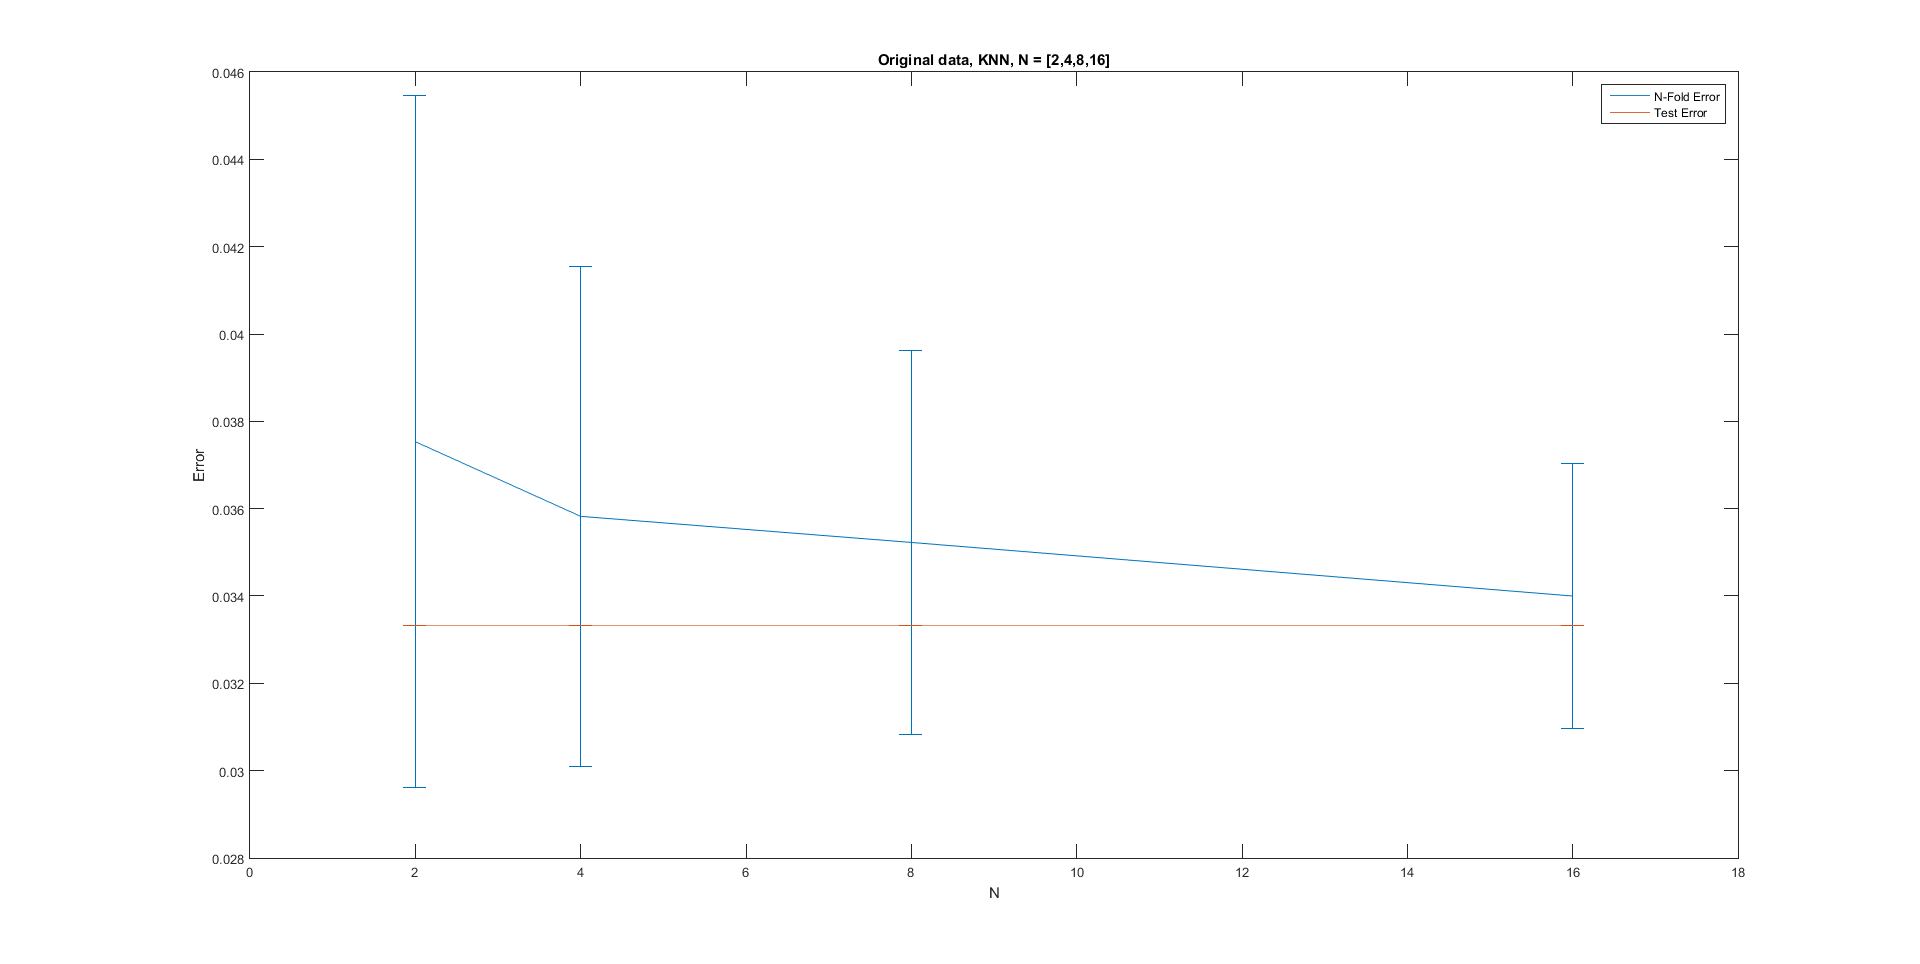
\includegraphics[width=7in, height=3in]{knn_OG_varyN.png}
\end{figure}
 
Noisy data with KNN
\begin{figure}[H]
\centering
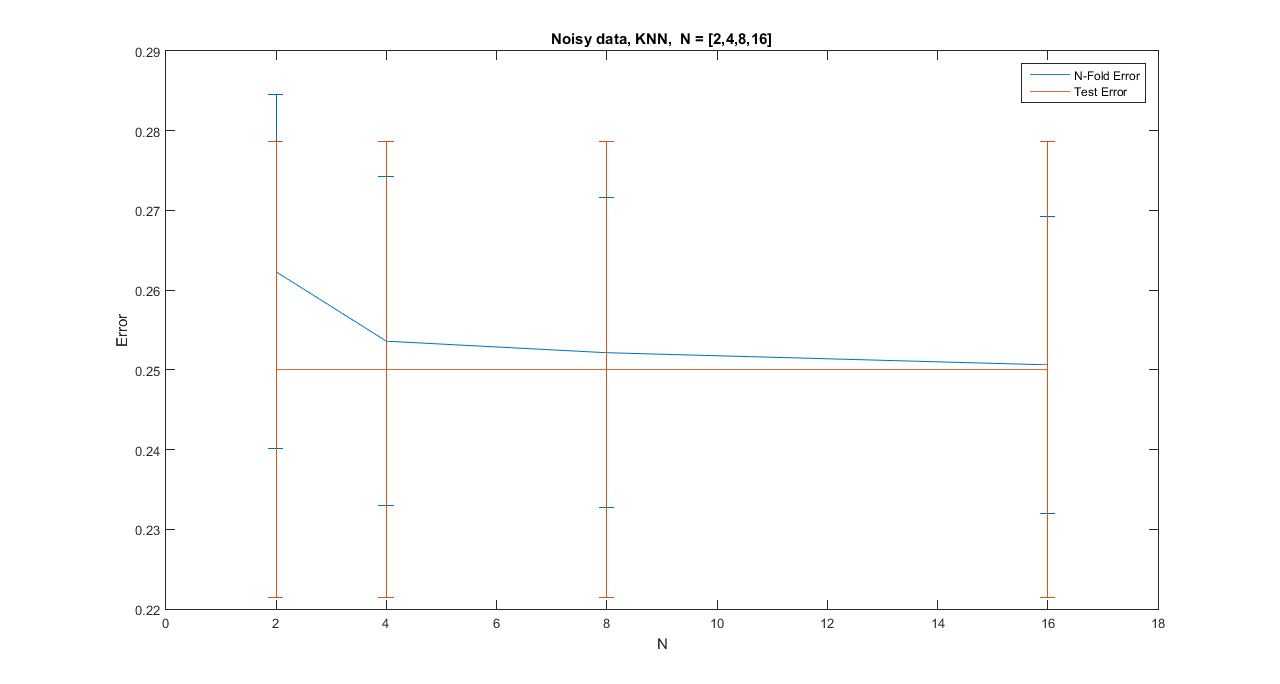
\includegraphics[width=7in, height=3in]{knn_noisy_varyN.png}
\end{figure}
 
Original data with Kernel Regression
\begin{figure}[H]
\centering
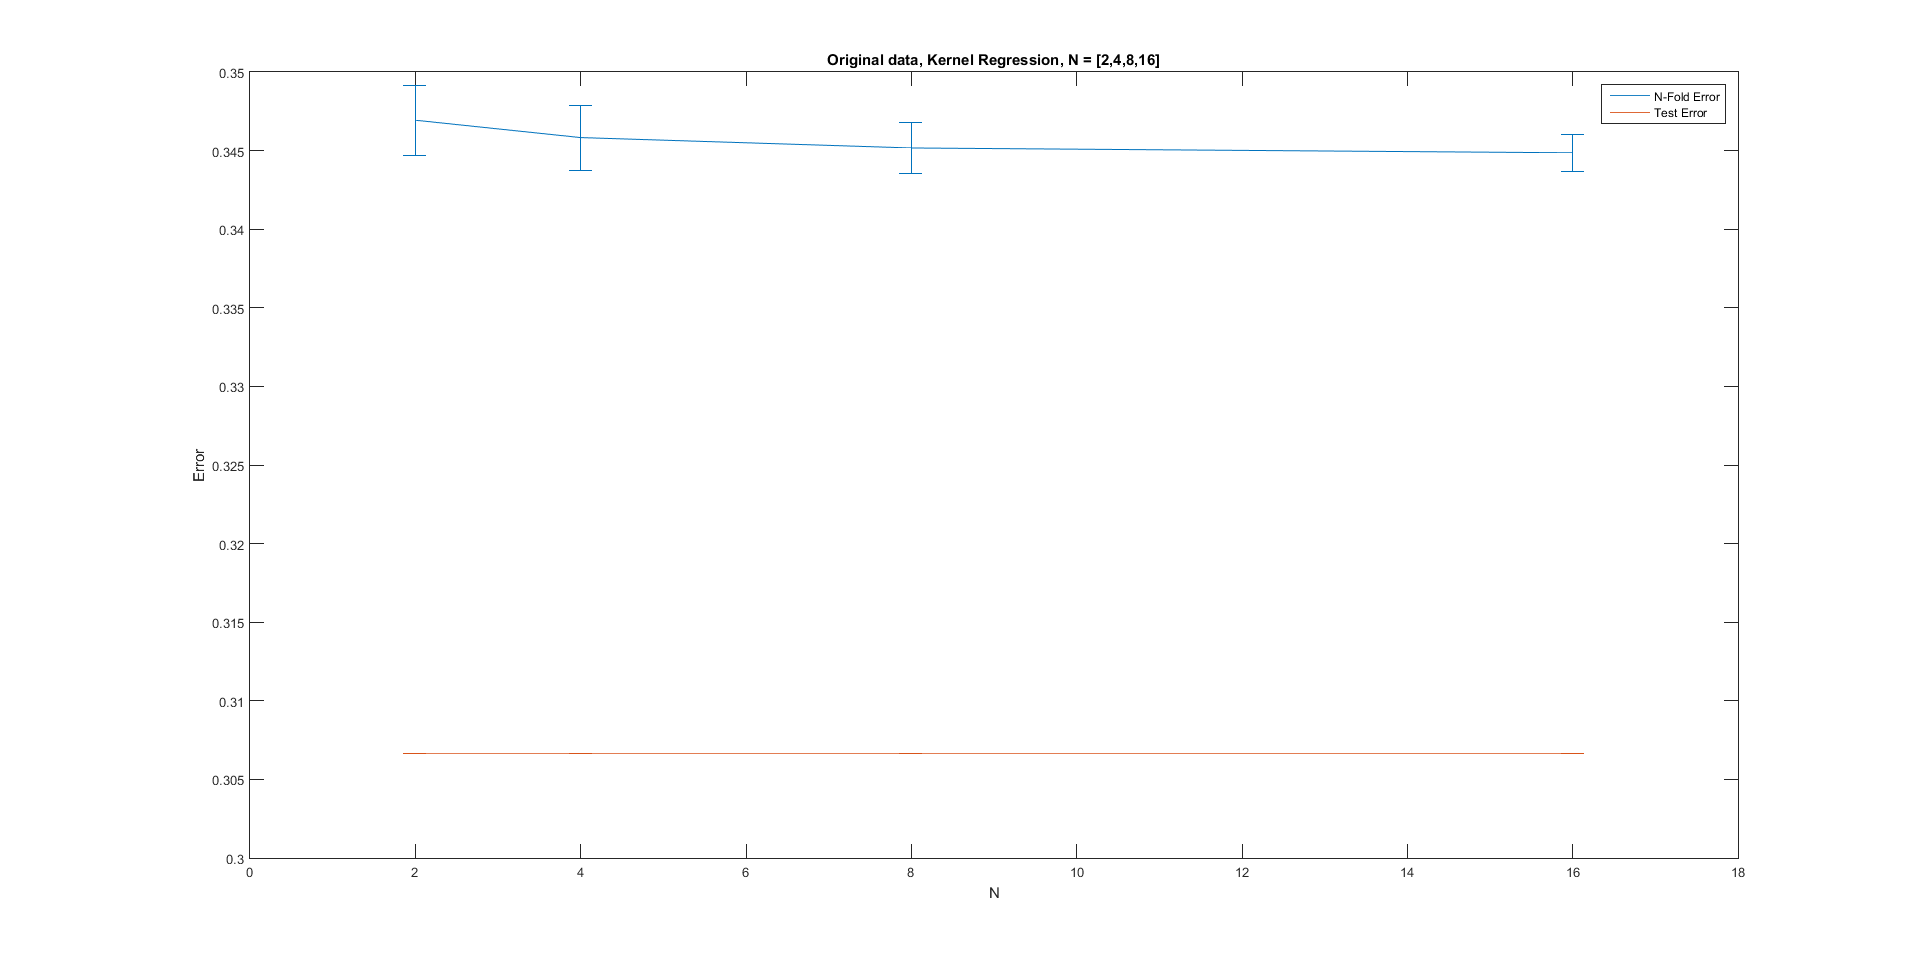
\includegraphics[width=7in, height=3in]{kern_OG_varyN.png}
\end{figure}

Noisy data with Kernel Regression
\begin{figure}[H]
\centering
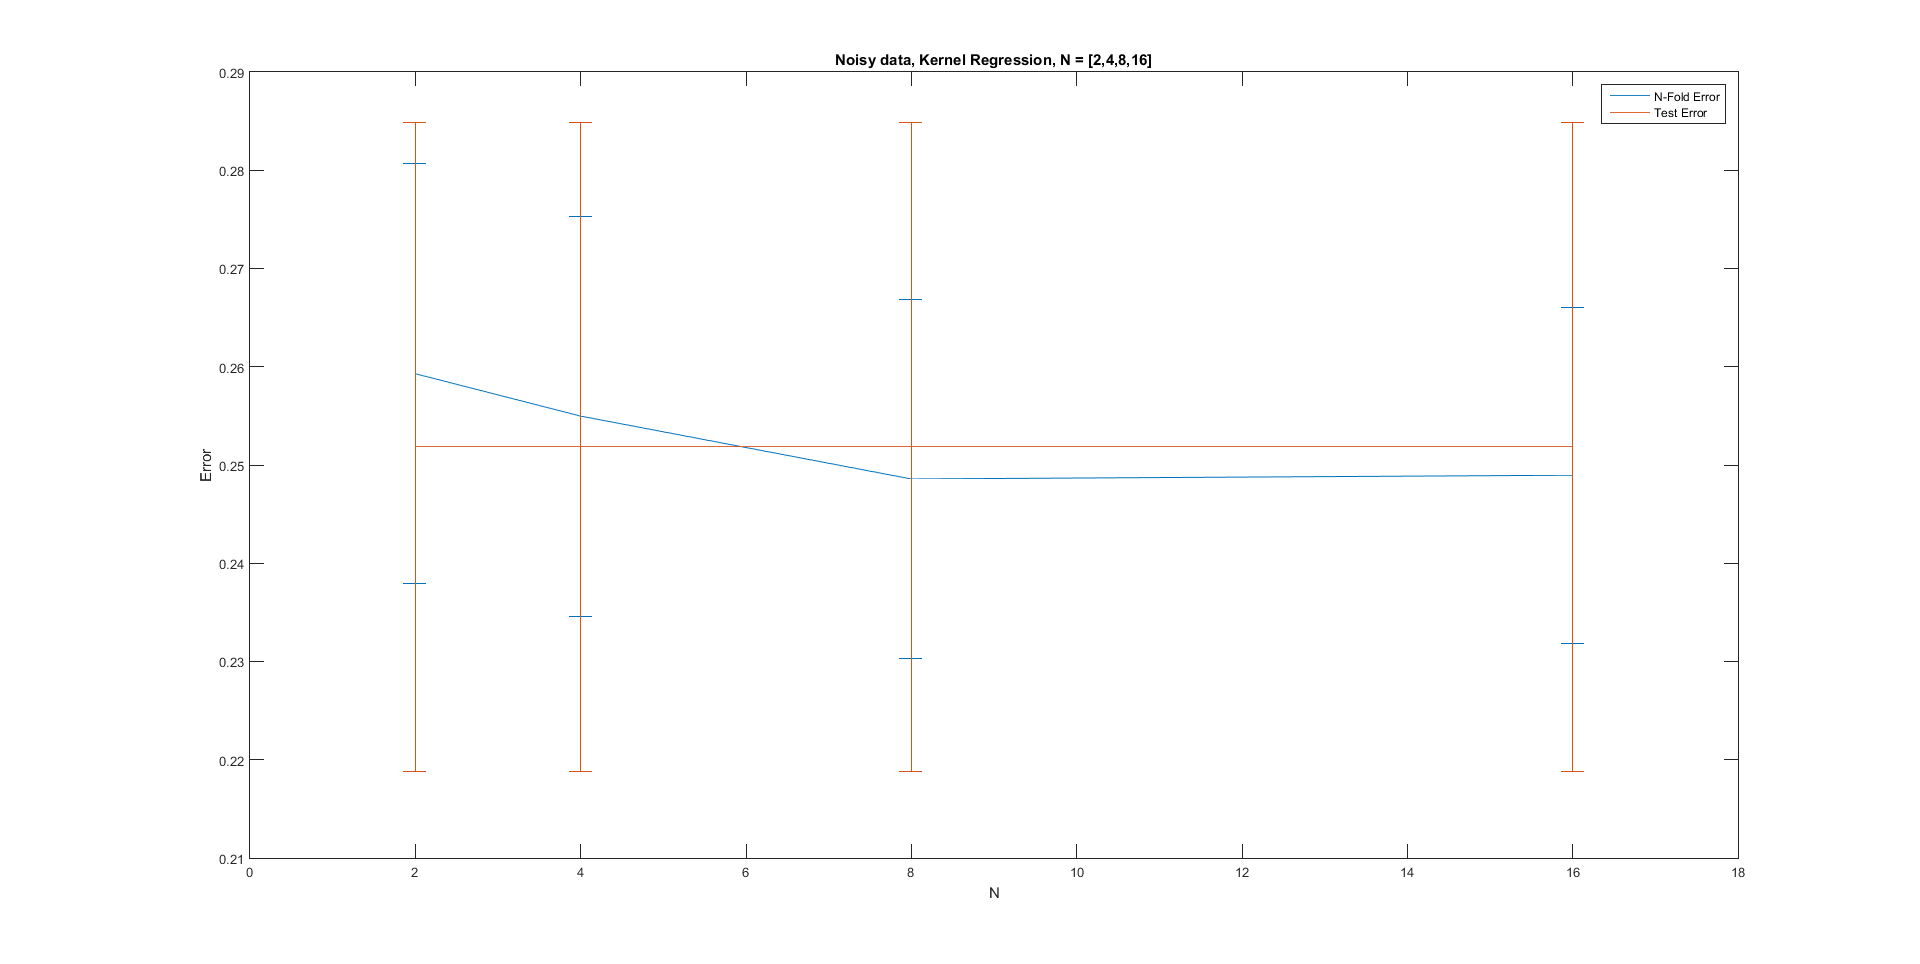
\includegraphics[width=7in,height=3in]{kern_noisy_varyN.png}
\end{figure}

In general, the training error and the testing error are very close and do not get better as $N$ increases. It is worth noting that the training and testing error for the noisy datasets are much larger than those using the original data. 

 
\item For both the original and the noisy data, compute the
  10-fold cross validation error on the training set and the corresponding test error for K-NN with
  $K \in \{1, 2, 3, 5, 8, 13, 21, 34\}$ and for Kernel Regression with $\sigma \in \{1, 2, 3,\ldots, 12\}$.  Generate {\bf
    four plots}: each plot will show $K$ (for K-NN) or $\sigma$ (for
  kernel regression) on the X axis, and error on the Y axis. The plot
  will have two lines, one for 10-fold error, and the
  other for test set error; you will have one plot for each
  method/dataset combination (e.g., K-NN on standard, K-NN on noisy,
  etc.). Based on these charts, can you pick the best $\sigma$ and $K$
  to minimize test set error using cross validation (on average) for both original and noisy data? Which are the best values? 
  
\paragraph{Your answer:}
 ~\\

Original data with KNN
\begin{figure}[H]
\centering
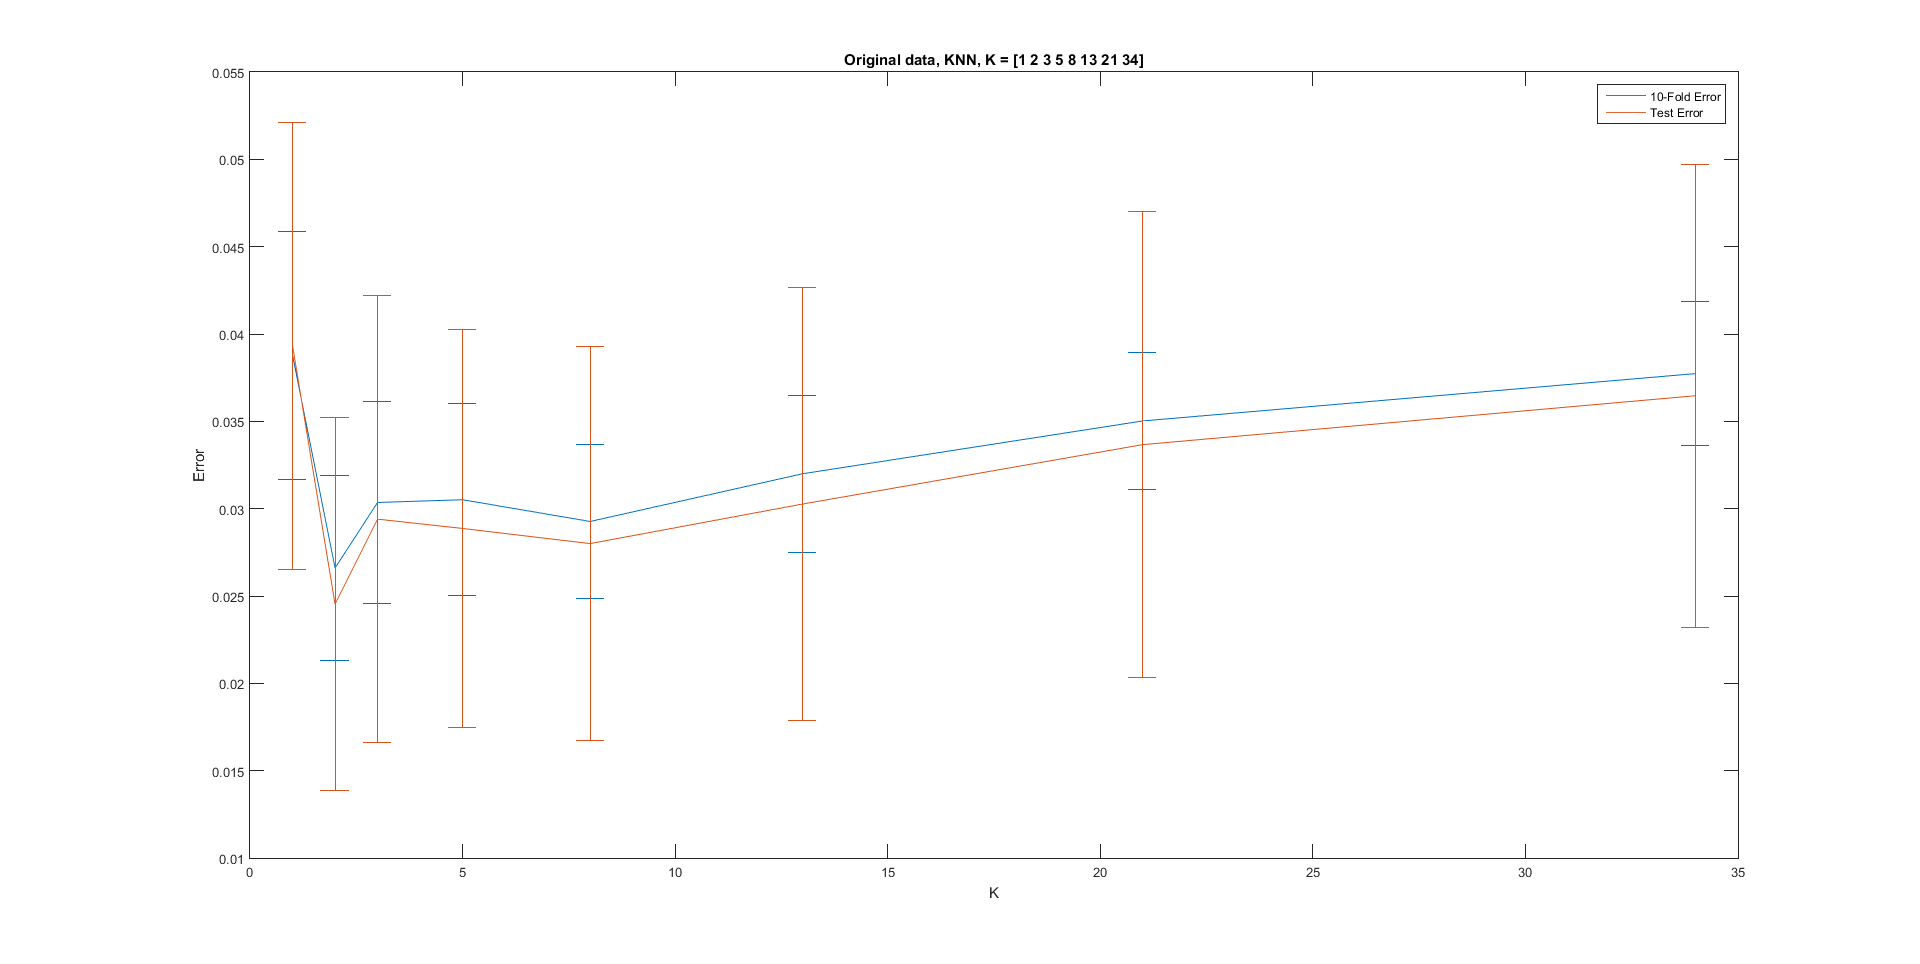
\includegraphics[width=7in, height=3in]{knn_OG_varyK.png}
\end{figure}

Noisy data with KNN
\begin{figure}[H]
\centering
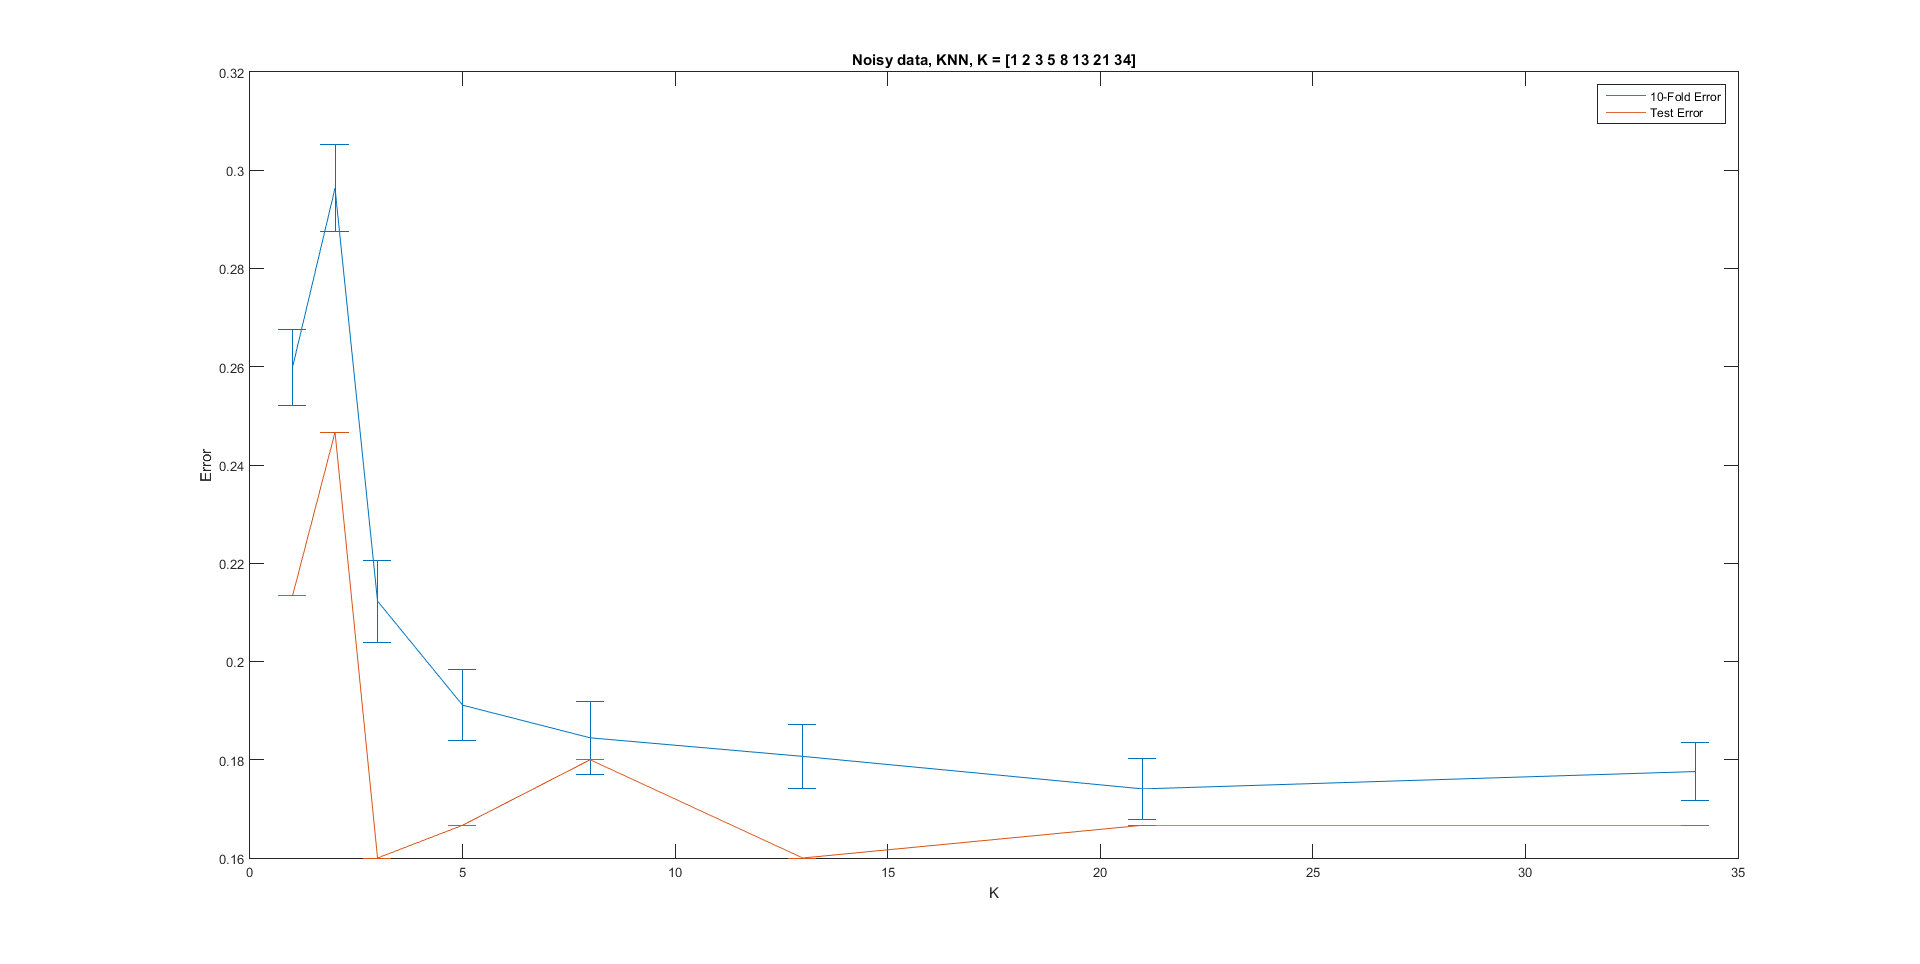
\includegraphics[width=7in, height=3in]{knn_noisy_varyK.png}
\end{figure}

Original data with Kernel Regression
\begin{figure}[H]
\centering
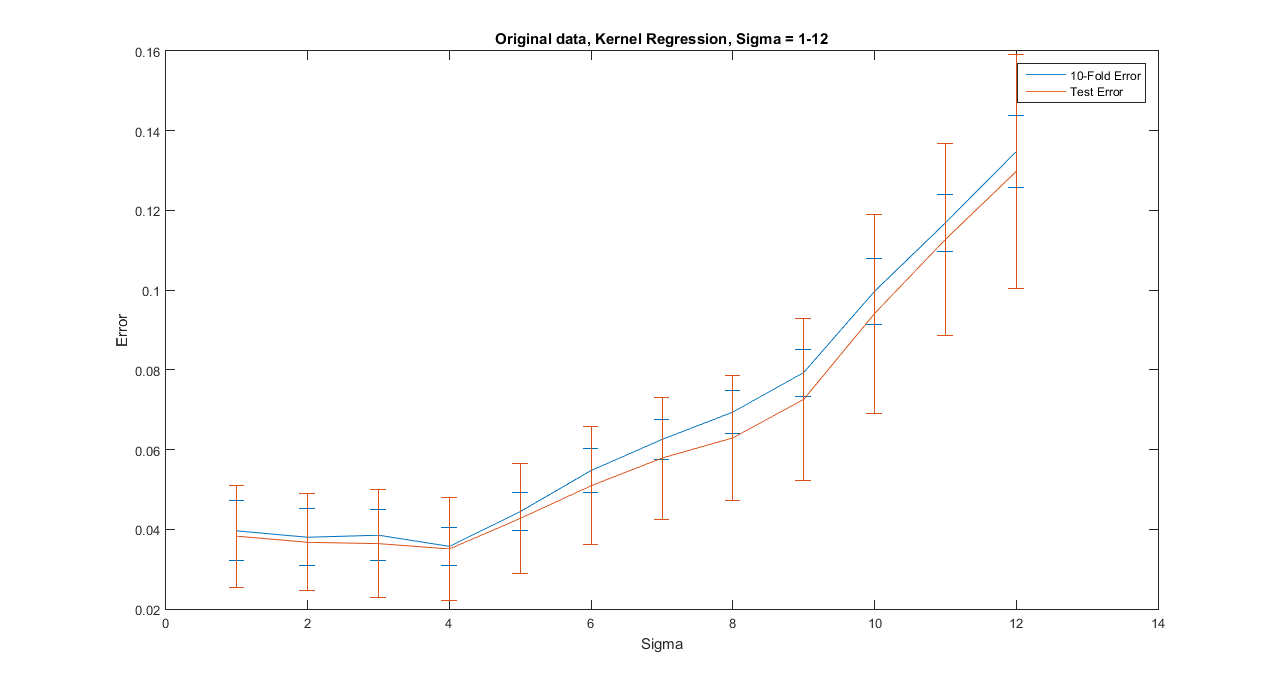
\includegraphics[width=7in, height=3in]{kern_OG_varySIGMA.png}
\end{figure}

Noisy data with Kernel Regression
\begin{figure}[H]
\centering
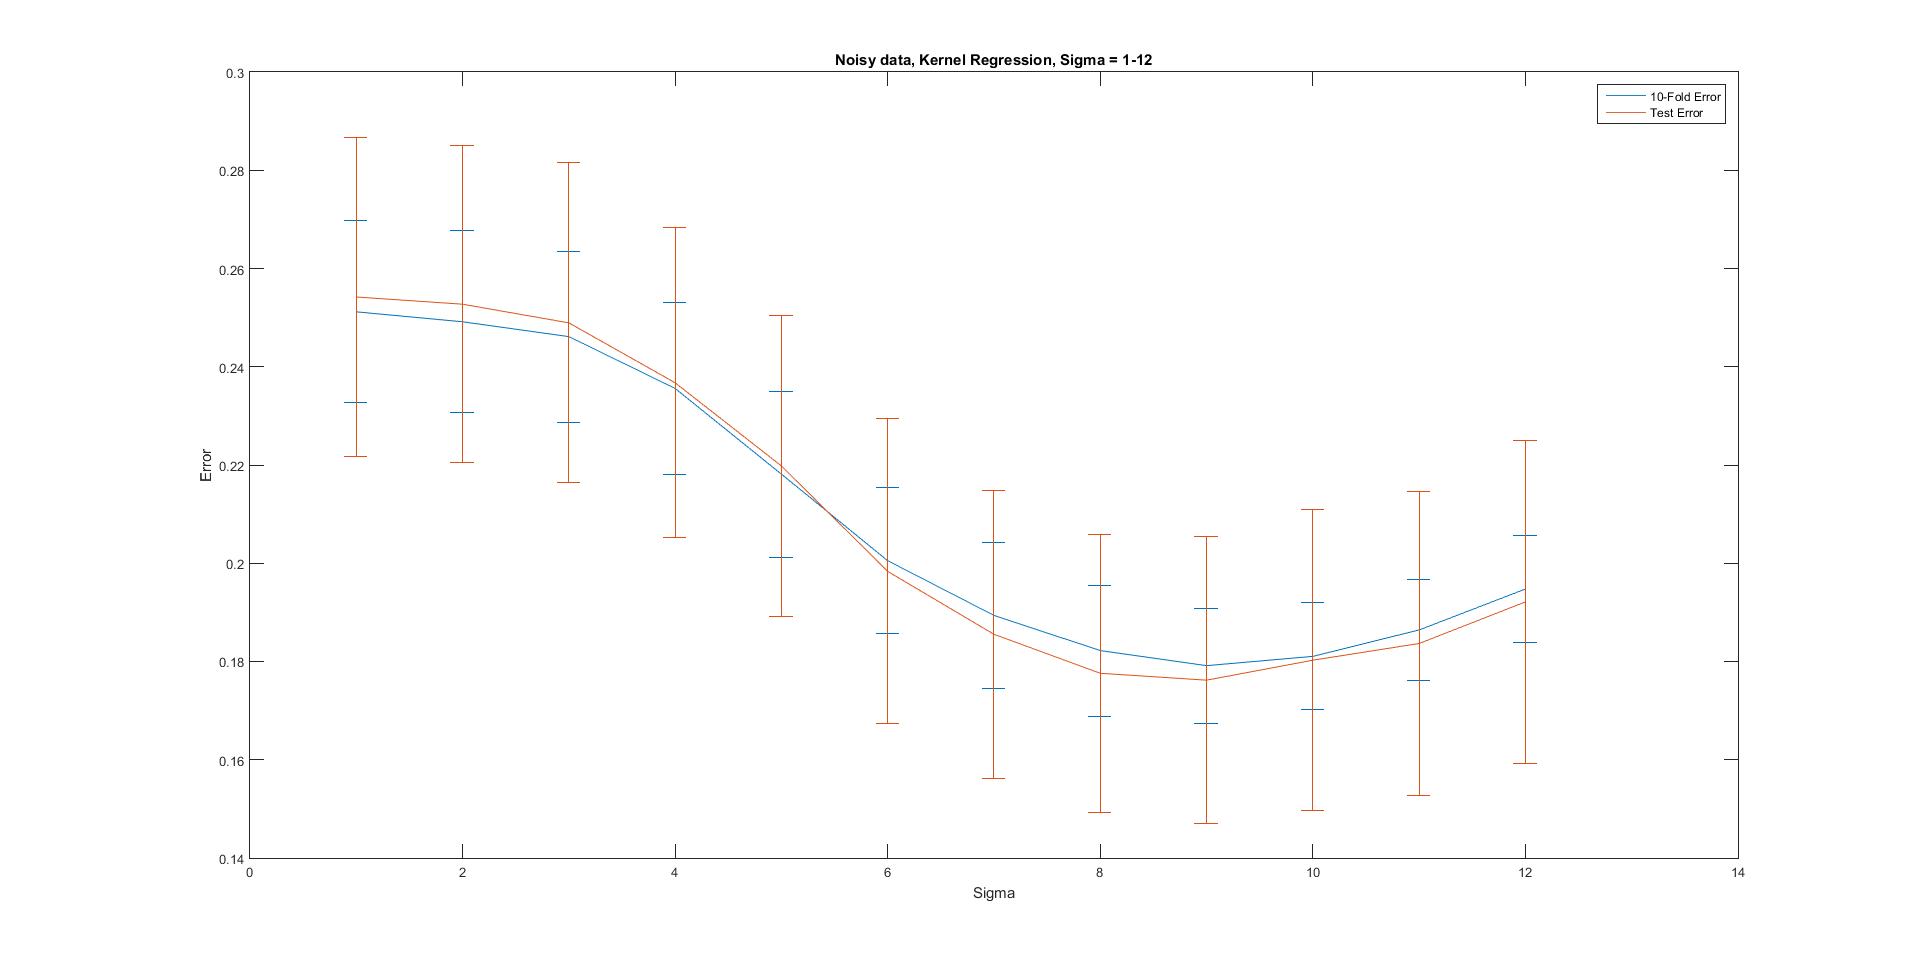
\includegraphics[width=7in, height=3in]{kern_noisy_varySIGMA.png}
\end{figure}
 
 The best $\sigma$ for the original data is 4, the best $\sigma$ for the noisy data is 9, the best $K$ for the original data is 2, and the best $K$ for the noisy data is 34.


\end{itemize}

\emph{\textsc{N-fold error and test error clarification:} N-fold error is the error over the training set, and test error is the error when you test your trained classifier (trained over the entire training set) on test set. N-fold cross validation is used for choosing the best parameters. }

 {\bf Note that any two random partitions of the data will yield somewhat different curves. Therefore, you must repeat all of the above steps 100 times, using different random partitions into training and testing.}

\section{Logistic Regression \hpoints{40}}

\paragraph{Description.} In this part, you will implement a very useful binary classifier {\tt Logistic Regression} to work with the task in Problem 2 and compare the results with some other methods. 


 Logistic Regression is a classifier used to estimate the probability that a given example belongs to a specific class based on features. These probabilities are estimated based on $\langle w,x\rangle$, where $x$ is a feature vector of an observation whose label is to be predicted, and $w$ is a vector of weights, with each coordinate of the vector corresponding to a feature of $x$. Unfortunately, these is no closed form expression for computing this weight vector $w$ which can minimize the loss function over the set of observations and labels (on training set). Luckily for us, this loss function is concave, thus allowing us to implement a powerful optimization technique called gradient ascent. Your task in this section is to implement the functions {\tt gradient\_ascent\_fixed.m}, {\tt gradient\_ascent\_decay.m}, {\tt logistic\_regression.m}, {\tt logistic\_xval\_error.m}
({\bf see each file for exact specifications}):


\begin{itemize}
\item {\tt gradient\_ascent\_fixed.m}. In this function, you shall implement the vanilla gradient ascent algorithm, with a constant step size (update rate in the lecture). In gradient ascent, the choice of step size is crucial, and in this section, you shall explore its effect on the performance of your algorithm. You will have to experiment a little with the choice of the step size to ensure good performance. Set the step size to a value you found to work best empirically. 

\item {\tt gradient\_ascent\_decay.m} Implement gradient ascent with step size that decays over time. You will have to experiment a little with the choice of the initial step size to ensure good performance. Did you notice any improvement over your implementation of gradient ascent with a decaying step size? What do you think was the cause of the improvement? Plot the evolution of the zero-one loss over training data as the gradient ascent proceeds i.e. plot the training error on the Y axis, and iterations on the X axis for both implementations of gradient ascent (fixed step size and decaying step size) in the same plot. Do this for both the noiseless and noisy dataset.

\paragraph{Your answer:}
 ~\\
 
 {\tt  [Figure on original data]}
 \\    
 
 {\tt [Figure on noisy data]}
 \\
  
  There is an improvement because \ldots  
  \\

\item Add an extra feature to your data that is always set to 1, and perform gradient ascent on this new data. This corresponds to adding a constant to the scores, i.e. $\langle w,x\rangle + c$. Did you notice any improvement in performance? What do you think happened that caused this improvement? Plot the evolution of the zero-one loss over training data as the gradient ascent proceeds i.e. plot the training error on the Y axis, and iterations on the X axis over the data without the extra feature, and with the extra feature in the same plot. Do this for both the noiseless and noisy dataset.

\paragraph{Your answer:}
 ~\\
 
 {\tt  [Figure on original data]}
 \\    
 
 {\tt [Figure on noisy data]}
 \\
  
 There is an improvement because \ldots  
  \\

\item Implement {\tt logistic\_regression.m} and {\tt logistic\_xval\_error.m}. For both the original data and the noisy, compute both the $N$-fold error on the training set, for $N = \{2, 4, 8, 16\}$, and the test error. What trend do you observe? Please plot the cross-validation error and test error in the same figure.

\paragraph{Your answer:}
 ~\\
 
 {\tt  [Figure on original data]}
 \\    
 
 {\tt [Figure on noisy data]}
 \\
  

\end{itemize}

\section{Method comparison \hpoints{10}}

You now have implemented several powerful tools to do binary
classfication, e.g. Logistic Regression, K-NN and kernel regression.
We also provide you a decision tree tool in the code.

\begin{itemize}

\item Please use each of these tools to compute the training error and testing error on both original and noisy data. You should fill in the table as follows. (Please use the best parameter you have found in K-NN, kernel regression and Logistic Regression.)

%{\it This problem (only) should be submitted on canvas; one copy per programming team}

\begin{table}[!htb]
\centering
\begin{tabular}{|c|c|c|c|c|c|} \hline
&training error on $X$& testing error on $X$&training error on $X_{\text noisy}$&testing error on $X_{\text noisy}$\\ \hline
K-NN & 0.0222 & 0.0200 & 0.1800 & 0.1267 \\ \hline
Kernel Regression & 0.0422 & 0.0133 & 0.1844 & 0.1267 \\ \hline
Decision Tree & & & & \\ \hline
Logistic Regression & & & & \\ \hline
\end{tabular}
\end{table} 

\item Then use one or two sentences to describe your idea on these methods respectively including their advantages and disadvantages based on the comparison. 

\paragraph{Your answer:}
 ~\\
 
\end{itemize}
\end{document}
